\documentclass[11pt]{exam}
\RequirePackage{amssymb, amsfonts, amsmath, latexsym, verbatim, xspace, setspace}
\RequirePackage{tikz, pgflibraryplotmarks}
\usepackage[margin=1in]{geometry}


\newcommand{\class}{MATH 241 - FALL 2024}
\newcommand{\examnum}{Midterm 2}
\newcommand{\examdate}{}
\newcommand{\timelimit}{75 Minutes}
\usepackage{tikz}
\usepackage{amsmath}
\usetikzlibrary{arrows}
\usepackage{tkz-euclide}
\usepackage{pgfplots}
\singlespacing
\parindent 0ex

\begin{document}
\pagestyle{head}
\firstpageheader{}{}{}
\runningheader{\class}{\examnum\ - Page \thepage\ of \numpages}{\examdate}
\runningheadrule
\begin{flushright}
\begin{tabular}{p{2.8in} r l}
\textbf{\class} & \textbf{Name (Last, First):} & \makebox[2in]{\hrulefill}\\
\textbf{\examnum} &&\\
\textbf{Time Limit: \timelimit} & \textbf{Section:} & \makebox[2in]{\hrulefill}\\
\end{tabular}\\
\end{flushright}
\rule[1ex]{\textwidth}{.1pt}

% These commands set up the running header on the top of the exam pages
\pagestyle{head}
\firstpageheader{}{}{}
\runningheader{\class}{\examnum\ - Page \thepage\ of \numpages}{\examdate}
\runningheadrule

\begin{flushleft}
\begin{center}

\end{center}
\end{flushleft}

\hfill
\begin{minipage}[t]{4.3in}
\vspace{0pt}
%\cellwidth{3em}
\gradetablestretch{1.4}
\vqword{Problem}
\addpoints % required here by exam.cls, even though questions haven't started yet.	
\gradetable[v]%[pages]  % Use [pages] to have grading table by page instead of question



\end{minipage}

\begin{flushleft}
\vspace{0.5in}
\textbf{Instructions:}
\begin{itemize}
    \item Write your full name (Last, First) and Section number above.
    \item Answer all the questions below and show your work.
    \item No electronic devices (including calculators) are to be used during the exam.
    \item The exam is closed book and closed notes.
    \item\textbf{Do not use L'H\^{o}pital's rule anywhere on this exam.}
    \item Turn in your exam at the end of the allotted time.
\end{itemize}
\textbf{Good Luck!}

\vspace{0.75in}
\textbf{Sign below to acknowledge that you have read and agree to the above instructions.}

\vspace{0.35in}
Signature: \makebox[5.5in]{\hrulefill}\\
\end{flushleft}

\newpage

\begin{questions}
\addpoints

\question %1
Consider $f(x)=\sqrt[4]{5x-4}$. Notice that $f(4)=\sqrt[4]{16}=2$.
\begin{parts}
\part[6] Write an equation of the line which is tangent to $f(x)$ at the point $(4,2)$.
\vfill
\part[4] Use your answer from above to approximate $\sqrt[4]{12}$ as a decimal or fraction.
\vfill
\end{parts}
\newpage

\question[10] %2
Find the absolute maximum and the absolute minimum of the function
$$f(x)=10x\sqrt{3-5x}$$ for $-1\leq x\leq \frac{3}{5}$ or else say why they don't exist. Your final answer needn't be fully simplified.
\newpage

\question %5
Determine the equation of the horizontal asymptote of the following functions.
\begin{parts}
    \part[4] $\displaystyle f(x)=\frac{2x^3}{x^3+5x^2-1}$
    \vfill
    \part[4] $\displaystyle g(x)=\frac{2x^3-3x^2+6x^4}{x-3x^5}$
    \vfill
\end{parts}
\newpage


\question%6
Consider the function $f(x) = x^4+4x^3-16x+3$.
\begin{parts}
    \part[5] Use the fact that $f'(x)=4(x-1)(x+2)^2$ to
    answer the following question: When is $f(x)$ decreasing?
    \vfill
    \part[5] Use the fact that $f''(x)=12x(x+2)$ to answer the following question: When is $f(x)$ concave down?
    \vfill
    
\end{parts}
\newpage


\question[8] %4
Decide whether or not $f(x)=\sqrt{x}-1$ satisfies the conditions of the Mean Value Theorem on the interval $[0,1]$. If not, briefly state what condition failed to be met and why. If so, find all values $c\in(a,b)$ so that the conclusion of the theorem $f'(c)=\frac{f(b)-f(a)}{b-a}$ holds.
\vfill
\question[6] Write down a function to be differentiated in order to answer the following optimization question. Do NOT solve the problem, only set up the function properly. Your answer should be given in terms of a single variable:

$\text{``You want to buy a rectangular poster board with an area }150\text{ square inches. You wish}$

$\text{to include }2\text{ inch margins along the top and along the bottom and }1\text{ inch margins along}$

$\text{both of the sides. What dimensions of the original poster board will give the largest}$

$\text{area within the margins?''}$

\vspace{6cm}




\newpage



\question %8
Imagine using Newton’s method to locate the zero values of the function $f(x)$ pictured below:
\begin{figure}[h!]
    \centering
    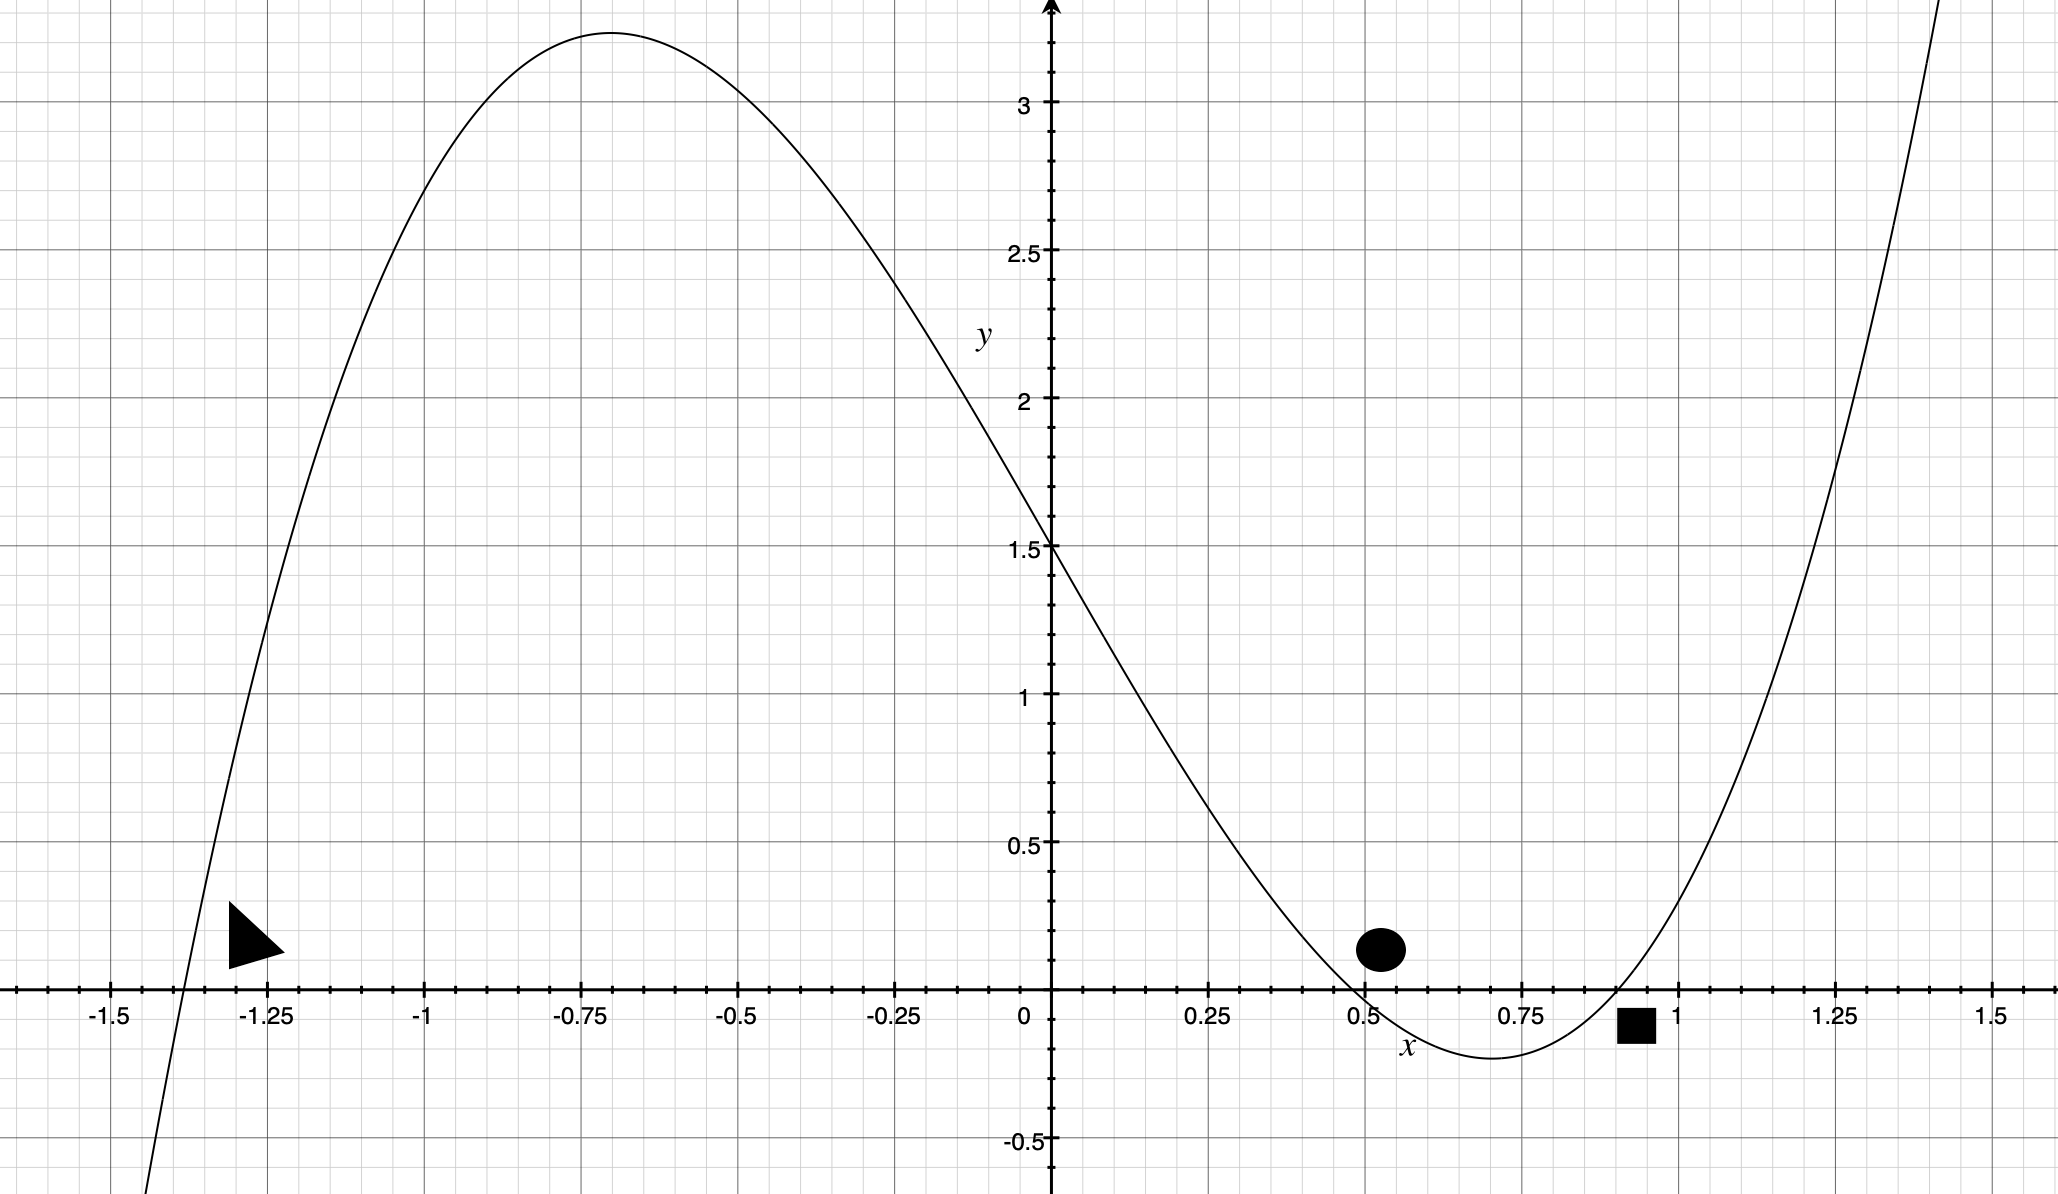
\includegraphics[scale=.45]{graph.png}
\end{figure}

\textbf{Hint: Carefully draw some of the tangent lines implicitly mentioned below in order to help you ``see" the answers.}
\begin{parts}
    \part[2] If you start with initial guess $x_0=-1.25$ to locate the root on the left (by the black triangle), will the updated guess $x_1$ be greater than or less than the true value?
    \vfill
    \part[2] If you start with initial guess $x_0=0.65$ to locate the root in the middle (by the black circle), will the updated guess $x_1$ be greater than or less than the true value?
    \vfill
    \part[2] If you start with initial guess $x_0=0.75$ to locate the root on the right (by the black square), will the updated guess $x_1$ be greater than or less than the true value?
    \vfill
\end{parts}
\newpage
\question Using $n=3$ rectangles and right endpoints, approximate the area under the curve shown below: $f(x)=4-x^2$ between $0\leq x\leq 1.5$. 
\begin{parts}
    \part[8] For full credit, clearly draw the three rectangles and write down the corresponding Riemann sum (you don't have to calculate the sum.)
\begin{figure}[h!]
    \centering
    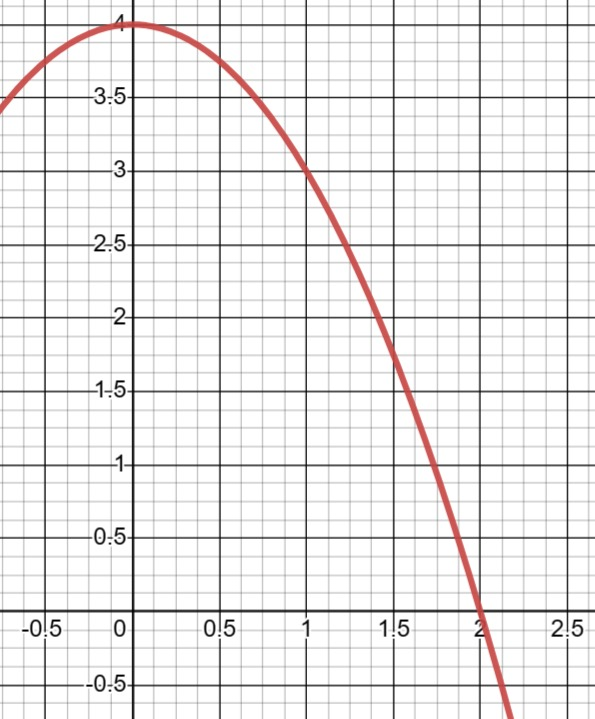
\includegraphics[scale=.5]{Images/S23 M215 PMT3 pic1.jpeg}
\end{figure}
\vfill
\part[2] Is your approximation an over estimate or an under estimate?
\vspace{2cm}
\end{parts}




\newpage
\question
Use the graphs provided and properties of definite integrals to determine whether the value is either positive, negative, or zero (circle one).
\begin{parts}
    \part[2] $\displaystyle\int_{-\pi/2}^{\pi/2}\sin(x)dx$
    \hspace{15mm}
    $\text{A.) Positive}$
    \hspace{5mm}
    $\text{B.) Negative}$
    \hspace{5mm}
    $\text{C.) Zero}$
\begin{figure}[h!]
\raggedleft
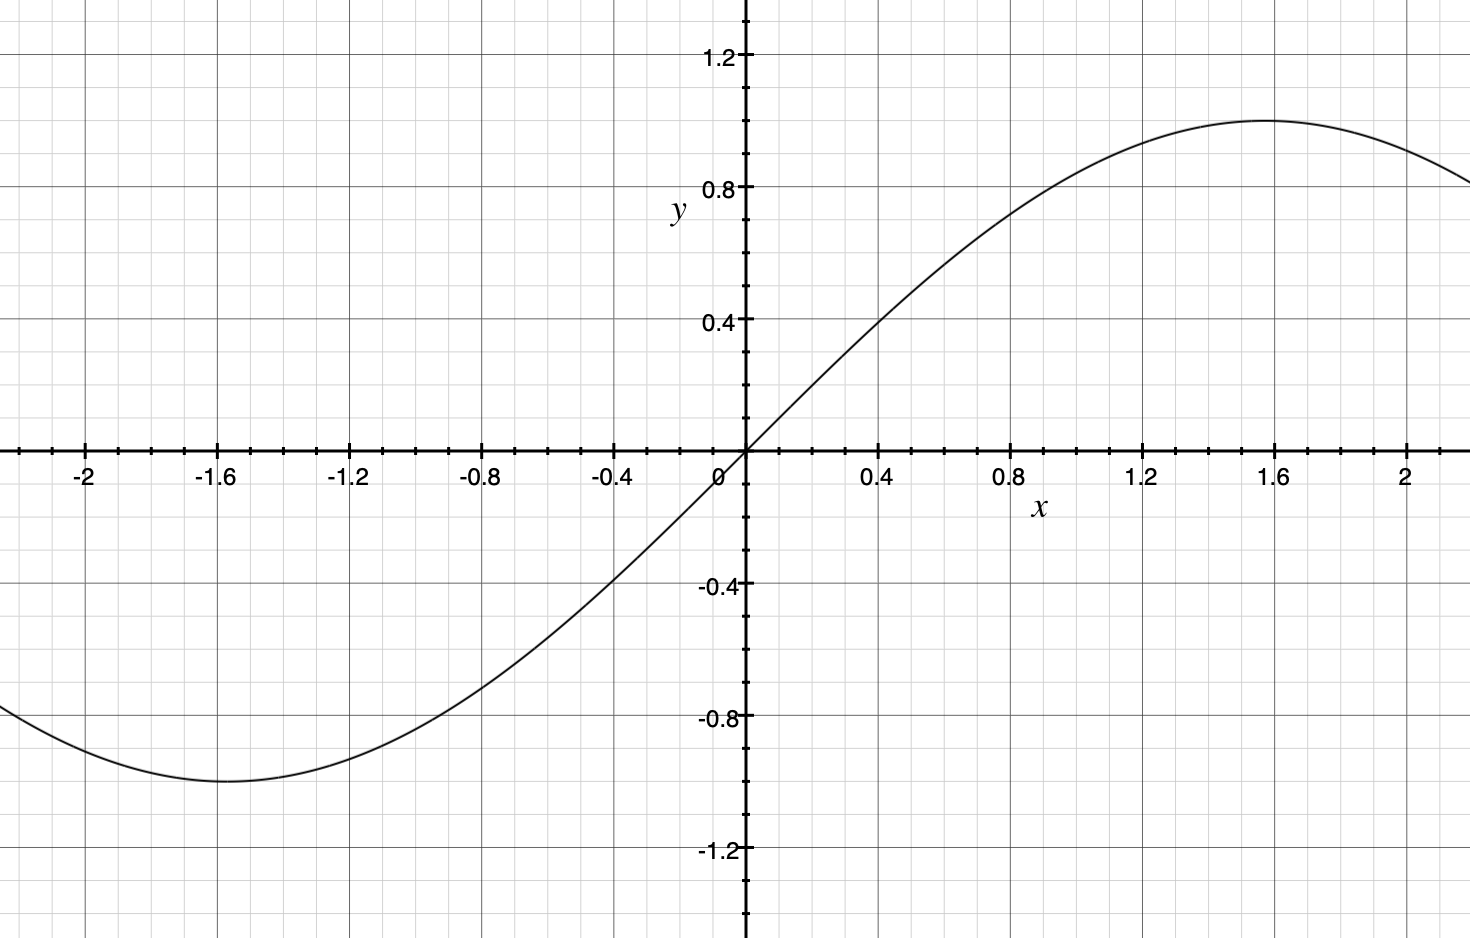
\includegraphics[scale=.3]{sin.png}
\end{figure}
    \part[2] $\displaystyle\int_{-0.5}^{1}-x^3dx$
    \hspace{15mm}
    $\text{A.) Positive}$
    \hspace{5mm}
    $\text{B.) Negative}$
    \hspace{5mm}
    $\text{C.) Zero}$
\begin{figure}[h!]
\raggedleft
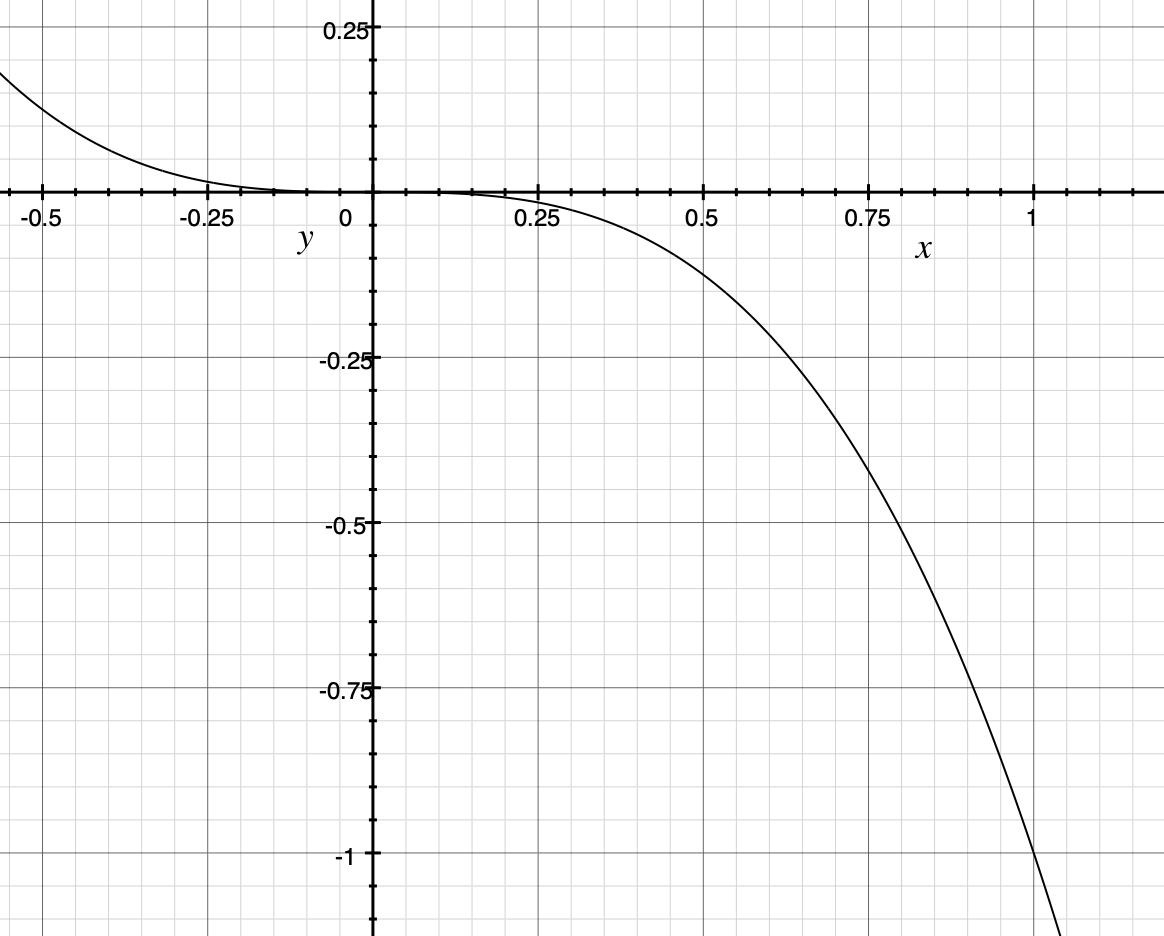
\includegraphics[scale=.3]{cubic.png}
\end{figure}
    \part[2] $\displaystyle\int_{0.8}^{-2}\frac{x^5}{50}dx$
    \hspace{15mm}
    $\text{A.) Positive}$
    \hspace{5mm}
    $\text{B.) Negative}$
    \hspace{5mm}
    $\text{C.) Zero}$
\begin{figure}[h!]
\raggedleft
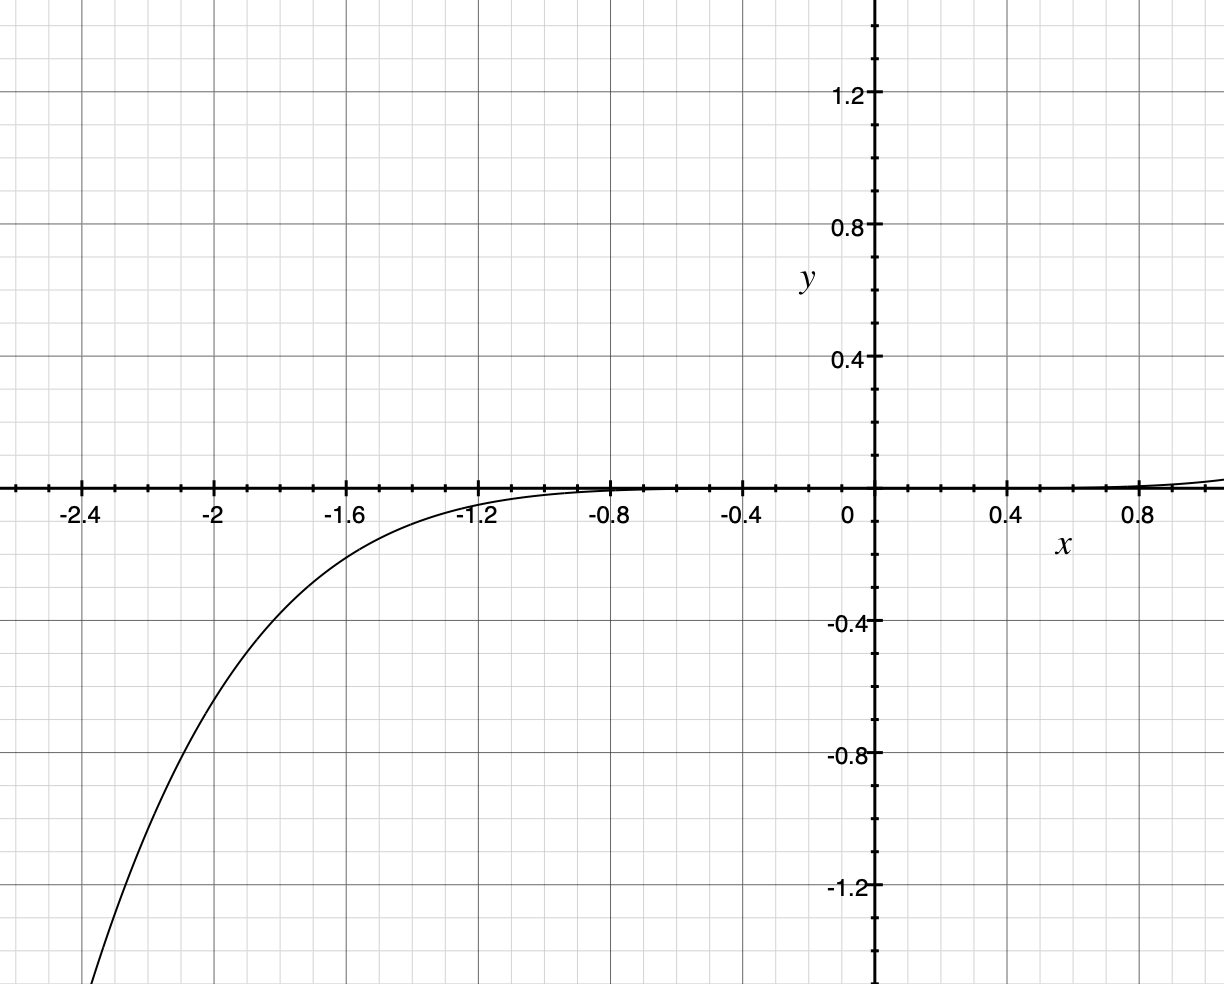
\includegraphics[scale=.3]{x5.png}
\end{figure}    
    
\end{parts}

\newpage
\question[6] Find the function $f(x)$ that satisfies the given condition:
$$f'(x)=2x-3\cos(x)\text{ and }f(0)=2$$
\vfill


\end{questions}
\end{document}
